\section*{Problema P9.37}

\begin{center}
    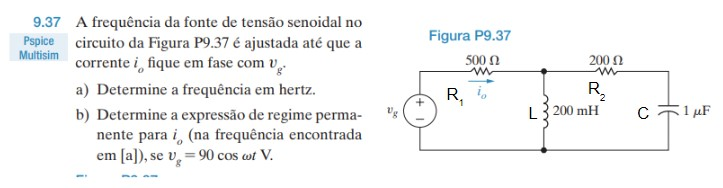
\includegraphics[scale=1.0]{P9.37.jpg}
\end{center}

\subsection*{(a)}

Vamos começar identificando a impedância equivalente \( Z_{in} \) vista pela fonte \( v_g \).

\[ Z_{in} = \left(\left(\frac{1}{j\omega C} + R_2\right) \; // \; j\omega L\right) +  R_1 \]

\[ Z_{in} = R_1 + \frac{1}{\frac{1}{j\omega L} + \frac{1}{\frac{1}{j\omega C} + R_2}}  \]

Agora vamos isolar a parte real da parte complexa.

\[ Z_{in} = R_1 + \frac{1}{-\frac{j}{\omega L} + \frac{1}{-\frac{j}{j\omega C} + R_2}}  \]

\[ Z_{in} = R_1 + \frac{1}{-\frac{j}{\omega L} - \frac{j\omega C}{j + jR_2j\omega C}}  \]

\[ Z_{in} = R_1 + \frac{1}{-\frac{j}{\omega L} - \frac{\omega C}{1 + jR_2\omega C}}  \]

\[ Z_{in} = R_1 + \frac{1}{-\frac{j}{\omega L} - \frac{\omega C(1 - jR_2\omega C)}{1^2 + (R_2\omega C)^2}}  \]

\[ Z_{in} = R_1 + \frac{1}{-\frac{j}{\omega L} - \frac{\omega C}{1 + R_2^2\omega^2 C^2} + j\frac{R_2\omega^2 C^2}{1 + R_2^2\omega^2 C^2}}  \]

\[ Z_{in} = R_1 + \frac{1}{- \frac{\omega C}{1 + R_2^2\omega^2 C^2} + j\left(-\frac{1}{\omega L} + \frac{R_2\omega^2 C^2}{1 + R_2^2\omega^2 C^2}\right)}  \]

\[ Z_{in} = R_1 + \frac{- \frac{\omega C}{1 + R_2^2\omega^2 C^2} - j\left(-\frac{1}{\omega L} + \frac{R_2\omega^2 C^2}{1 + R_2^2\omega^2 C^2}\right)}{(\frac{\omega C}{1 + R_2^2\omega^2 C^2})^2 + \left(-\frac{1}{\omega L} + \frac{R_2\omega^2 C^2}{1 + R_2^2\omega^2 C^2}\right)^2}  \]

Vamos adotar uma notação para simplificar a expressão. Sejam

\[ 
    A = \frac{\omega C}{1 + R_2^2\omega^2 C^2}
    \quad , \quad
    B = -\frac{1}{\omega L} + \frac{R_2\omega^2 C^2}{1 + R_2^2\omega^2 C^2}
\]

Com isso, podemos reescrever a expressão de \( Z_{in} \) como

\[ Z_{in} = R_1 + \frac{- A - jB}{A^2 + B^2}  \]

\[ Z_{in} = \left(R_1 - \frac{A}{A^2 + B^2}\right) - j\frac{B}{A^2 + B^2}  \]

Agora é possível epxressar uma função para o ângulo de fase \( \phi \) de \( Z_{in} \), dada por

\[ \phi = \tan^{-1}\left(\frac{\frac{B}{A^2 + B^2}}{R_1 - \frac{A}{A^2 + B^2}}\right) \]

\[ \phi = \tan^{-1}\left(\frac{\frac{B}{A^2 + B^2}}{\frac{R_1(A^2 + B^2) - A}{A^2 + B^2}}\right) \]

\begin{equation}\label{eq:9.37-1}\tag{9.37-1}
    \phi = \tan^{-1}\left(\frac{B}{R_1(A^2 + B^2) - A}\right)
\end{equation}

Uma vez calculado $Z_{in}$, podemos expressar a relação entre $V_g$ e $I_o$ através de

\begin{equation}\label{eq:9.37-2}\tag{9.37-2}
    V_g = Z_{in} \cdot I_g
\end{equation}

Para que (\ref{eq:9.37-2}) seja satisfeita com $V_g$ e $I_o$ em fase, temos que o ângulo de fase de $Z_{in}$ deve ser nulo. Portanto, usando (\ref{eq:9.37-2}), temos

\[ \phi = \tan^{-1}\left(\frac{B}{R_1(A^2 + B^2) - A}\right) = 0 \]

\[ \frac{B}{R_1(A^2 + B^2) - A} = 0 \]

\[ B = 0 \]

Expandindo $B$ conforme o definimos, temos

\[ -\frac{1}{\omega L} + \frac{R_2\omega^2 C^2}{1 + R_2^2\omega^2 C^2} = 0 \]

\[ \frac{-(1 + R_2^2\omega^2 C^2) + (\omega L)(R_2\omega^2 C^2)}{(\omega L)(1 + R_2^2\omega^2 C^2)} = 0 \]

\[ -1 - R_2^2\omega^2 C^2 + (\omega L)(R_2\omega^2 C^2) = 0 \]

Isolando $\omega$, temos

\[ - R_2^2\omega^2 C^2 + \omega^3LR_2C^2 = 1 \]

\[ \omega^3LR_2C^2 - \omega^2R_2^2C^2 - 1 = 0\]

Para solucionar a equação de 3° grau, vamos substituir os valores

\[ 4\cdot10^{-11}\omega^3 - 4\cdot10^{-8}\omega^2 - 1 = 0\]


Usando $\omega = 2\pi f$, a frequência $f$ em Hertz da fonte de tensão deve ser

\begin{equation}\label{eq:9.37-3}\tag{9.37-3}
    f = \frac{1}{2\pi}\frac{R_2}{L}
\end{equation}

Substituindo,

\[ \boxed{f = 159.15 \; \textrm{Hz}}  \]









